% Gabarit pandoc des corrigés publiés (brut et guidé). Contenu sans marque ni nom de site.
% Compilation : lualatex (latexmk -lualatex).
% Le Markdown reste la source unique : ne pas éditer ce fichier .tex à la main.
\documentclass[11pt,a4paper]{article}

% --- Moteur, polices (Latin Modern) et langue ---------------------------------
\usepackage{iftex}
\ifLuaTeX\else\errmessage{Ce document se compile avec lualatex}\fi
\usepackage{amsmath,amssymb,mathtools}
\usepackage{fontspec}
% mathrm=sym : \mathrm prend ses glyphes dans la police mathématique (ℓ, μ, Ω), comme KaTeX.
\usepackage[math-style=TeX,bold-style=TeX,mathrm=sym]{unicode-math}
% Repli pour les glyphes absents de Latin Modern (indices et exposants Unicode,
% flèches, filets des schémas en texte, symboles) : DejaVu, puis Latin Modern Math
% (ℓ, lettres mathématiques Unicode des légendes).
\directlua{
  luaotfload.add_fallback("repliTexte", {"DejaVuSerif:mode=harf;", "DejaVuSans:mode=harf;", "file:latinmodern-math.otf:mode=harf;"})
  luaotfload.add_fallback("repliMono", {"DejaVuSansMono:mode=harf;", "DejaVuSans:mode=harf;", "file:latinmodern-math.otf:mode=harf;"})
}
\setmainfont{Latin Modern Roman}[RawFeature={fallback=repliTexte}]
\setsansfont{Latin Modern Sans}[RawFeature={fallback=repliTexte}]
\setmonofont{Latin Modern Mono}[RawFeature={fallback=repliMono}]
\setmathfont{Latin Modern Math}
\usepackage[french]{babel}
\frenchsetup{SmallCapsFigTabCaptions=false}

% --- Mise en page --------------------------------------------------------------
\usepackage[a4paper,margin=2.2cm,headheight=14pt,footskip=1.2cm]{geometry}
\usepackage{microtype}
\setlength{\emergencystretch}{4em}
\tolerance=1500
\setlength{\parindent}{0pt}
\setlength{\parskip}{0.55\baselineskip plus 2pt minus 1pt}
\usepackage{xcolor}
% Gris nommés : babel-french rend « ! » actif dans le document.
\definecolor{gris2}{gray}{0.98}
\definecolor{gris3}{gray}{0.97}
\definecolor{gris5}{gray}{0.95}
\definecolor{gris35}{gray}{0.65}
\definecolor{gris40}{gray}{0.60}
\definecolor{gris45}{gray}{0.55}
\definecolor{gris50}{gray}{0.50}
\definecolor{gris55}{gray}{0.45}
\definecolor{gris60}{gray}{0.40}
\definecolor{gris65}{gray}{0.35}
\definecolor{gris70}{gray}{0.30}
\definecolor{gris80}{gray}{0.20}
\definecolor{gris85}{gray}{0.15}
\usepackage{graphicx}
\usepackage{float}
\usepackage{caption}
\captionsetup{font=small,labelformat=empty,justification=centering}
\usepackage{booktabs,longtable,array,multirow,calc}
\usepackage{siunitx}
\sisetup{locale=FR}
\usepackage[version=4]{mhchem}
\usepackage{listings}
\usepackage{fancyhdr}
\usepackage{lastpage}
\usepackage[most]{tcolorbox}
\usepackage{enumitem}
\setlist{nosep,leftmargin=*,topsep=2pt}
\usepackage[hidelinks,unicode]{hyperref}
\usepackage{bookmark}
\hypersetup{pdftitle={Agro-Véto BCPST — Mathématiques 2026},pdfauthor={Rédigé par IA},pdfcreator={LaTeX},pdfsubject={Corrigé brut}}
\usepackage{xurl}

% --- Pandoc : listes, tableaux, figures ----------------------------------------
\providecommand{\passthrough}[1]{#1}
\providecommand{\tightlist}{\setlength{\itemsep}{0pt}\setlength{\parskip}{0pt}}

\makeatletter
\def\maxwidth{\ifdim\Gin@nat@width>\linewidth\linewidth\else\Gin@nat@width\fi}
\def\maxheight{\ifdim\Gin@nat@height>0.55\textheight 0.55\textheight\else\Gin@nat@height\fi}
\makeatother
\setkeys{Gin}{width=\maxwidth,height=\maxheight,keepaspectratio}
\setcounter{secnumdepth}{-\maxdimen}
\providecommand{\pandocbounded}[1]{#1}

% --- Code (listings) -----------------------------------------------------------
\lstset{
  basicstyle=\ttfamily\small,
  columns=fullflexible,
  keepspaces=true,
  breaklines=true,
  breakatwhitespace=false,
  postbreak=\mbox{\textcolor{gris50}{$\hookrightarrow$}\space},
  frame=single,
  rulecolor=\color{gris35},
  framesep=4pt,
  xleftmargin=5pt,xrightmargin=5pt,
  backgroundcolor=\color{gris3},
  keywordstyle=\bfseries,
  commentstyle=\color{gris65},
  stringstyle=\color{gris80},
  showstringspaces=false,
  tabsize=4,
  extendedchars=true,
  aboveskip=6pt,belowskip=6pt,
}

% --- Macros des corrigés (KaTeX ↔ LaTeX) ---------------------------------------
% Les corrigés sont écrits pour KaTeX : on définit ici ce que KaTeX connaît et
% que LaTeX n'a pas, sans jamais retoucher le Markdown.
\providecommand{\R}{\mathbb{R}}
\providecommand{\N}{\mathbb{N}}
\providecommand{\Z}{\mathbb{Z}}
\providecommand{\Q}{\mathbb{Q}}
\providecommand{\C}{\mathbb{C}}
\providecommand{\dd}{\mathrm{d}}
\providecommand{\llbracket}{\lBrack}
\providecommand{\rrbracket}{\rBrack}
\providecommand{\lBrace}{\lbrace}
\providecommand{\rBrace}{\rbrace}
\providecommand{\Box}{\square}
\providecommand{\Diamond}{\lozenge}
\providecommand{\varnothing}{\emptyset}
\providecommand{\argmax}{\operatorname*{arg\,max}}
\providecommand{\argmin}{\operatorname*{arg\,min}}
\renewcommand{\leq}{\leqslant}
\renewcommand{\geq}{\geqslant}

% Équation hors texte : réduite à la largeur de la ligne si elle déborde.
\newsavebox{\boiteequation}
\newcommand{\equationajustee}[1]{%
  \sbox{\boiteequation}{$\displaystyle #1$}%
  \ifdim\wd\boiteequation>\linewidth
    \[\resizebox{\linewidth}{!}{\usebox{\boiteequation}}\]%
  \else
    \[#1\]%
  \fi}

% --- Encadrés pédagogiques (sobres, lisibles en noir et blanc) -----------------
\tcbset{
  encadre/.style={
    enhanced,breakable,sharp corners,
    colback=white,colframe=gris55,
    boxrule=0.4pt,leftrule=2.2pt,
    left=6pt,right=6pt,top=3pt,bottom=3pt,
    before skip=6pt,after skip=6pt,
    fonttitle=\bfseries\small,coltitle=black,
    attach title to upper,after title={\quad},
    parbox=false,
  }
}
\newtcolorbox{indication}[1]{encadre,colframe=gris45,colback=gris2,title={Indication~#1}}
\newtcolorbox{methode}{encadre,colframe=gris70,title={Méthode}}
\newtcolorbox{piege}{encadre,colframe=gris85,boxrule=0.8pt,leftrule=2.2pt,title={Piège}}
\newtcolorbox{jury}{encadre,colframe=gris60,colback=gris5,title={Jury}}
\newtcolorbox{encadrenote}{encadre,colframe=gris40}

% --- Titres de section ---------------------------------------------------------
\usepackage{titlesec}
\titleformat{\section}{\Large\bfseries}{}{0pt}{}
\titleformat{\subsection}{\large\bfseries}{}{0pt}{}
\titleformat{\subsubsection}{\normalsize\bfseries}{}{0pt}{}
\titlespacing*{\section}{0pt}{14pt plus 4pt minus 2pt}{6pt}
\titlespacing*{\subsection}{0pt}{10pt plus 3pt minus 2pt}{4pt}
\titlespacing*{\subsubsection}{0pt}{8pt plus 2pt minus 2pt}{2pt}

% --- En-tête et pied de page ---------------------------------------------------
\pagestyle{fancy}
\fancyhf{}
\fancyhead[L]{\small\textsc{Corrigé brut} · Agro-Véto BCPST}
\fancyhead[R]{\small Maths 2026}
\fancyfoot[L]{\footnotesize Corrigé rédigé par IA, non officiel}
\fancyfoot[R]{\footnotesize \thepage\,/\,\pageref*{LastPage}}
\renewcommand{\headrulewidth}{0.4pt}
\renewcommand{\footrulewidth}{0pt}
\fancypagestyle{plain}{\fancyhf{}\fancyfoot[R]{\footnotesize \thepage\,/\,\pageref*{LastPage}}\fancyfoot[L]{\footnotesize Corrigé rédigé par IA, non officiel}\renewcommand{\headrulewidth}{0pt}}

\begin{document}
\thispagestyle{plain}
\begin{center}
  {\small\scshape Corrigé brut}\par\smallskip
  {\LARGE\bfseries Agro-Véto BCPST — Mathématiques 2026\par}\medskip
  {\large Agro-Véto · BCPST · Maths · 2026\par}
\end{center}
\vspace{2pt}\hrule\vspace{8pt}

\emph{Corrigé rédigé par IA, non officiel. Signalez toute erreur.}

Épreuve « Méthodes de calcul et raisonnement », durée 2 h, sans calculatrice. Toutes les parties sont indépendantes, sauf la question 24.

\hypertarget{partie-i-approximation-de-la-loi-de-poisson}{%
\section{Partie I : Approximation de la loi de Poisson}\label{partie-i-approximation-de-la-loi-de-poisson}}

On suppose \(N\ge\lambda\), pour que \(\lambda/N\in\,]0,1]\) soit une probabilité. Cette hypothèse est sans conséquence, car on fait ensuite tendre \(N\) vers \(+\infty\).

\hypertarget{section}{%
\subsection{1.}\label{section}}

Pour \(i\in\{1,\dots,N\}\), notons \(B_i\) la variable qui vaut \(1\) si la \(i\)-ème bactérie devient résistante, et donc survit, et \(0\) sinon.

Chaque bactérie constitue une expérience de Bernoulli de succès « devenir résistante », de probabilité \(\lambda/N\). Les \(N\) expériences sont \textbf{mutuellement indépendantes}, par hypothèse de l'énoncé.

Le nombre \(X_N=\sum_{i=1}^N B_i\) de survivantes compte les succès dans \(N\) expériences de Bernoulli indépendantes de même paramètre. Donc \(X_N\) suit la loi binomiale :

\equationajustee{\boxed{X_N\sim\mathcal B\!\left(N,\tfrac{\lambda}{N}\right)}}

c'est-à-dire, pour tout \(k\in\{0,\dots,N\}\) :

\equationajustee{\boxed{\mathbb P(X_N=k)=\binom Nk\left(\frac\lambda N\right)^k\left(1-\frac\lambda N\right)^{N-k}.}}

\hypertarget{section-1}{%
\subsection{2.}\label{section-1}}

Soit \(k\in\mathbb N\) fixé. Pour \(N>\lambda\), on a \(0<1-\lambda/N<1\), d'où

\equationajustee{\left(1-\frac\lambda N\right)^{N-k}=\exp\!\left[(N-k)\ln\!\left(1-\frac\lambda N\right)\right].}

On étudie l'exposant. Quand \(N\to+\infty\), \(u_N=-\lambda/N\) tend vers \(0\), et \(\ln(1+u)\sim u\) en \(0\), donc :

\equationajustee{\ln\!\left(1-\frac\lambda N\right)\sim-\frac\lambda N .}

Comme \(k\) est fixé, \(N-k\sim N\). Par produit d'équivalents :

\equationajustee{(N-k)\ln\!\left(1-\frac\lambda N\right)\sim N\cdot\left(-\frac\lambda N\right)=-\lambda .}

Une suite équivalente à la constante non nulle \(-\lambda\) tend vers \(-\lambda\). L'exposant tend donc vers \(-\lambda\). Par continuité de l'exponentielle en \(-\lambda\) (composition de limites) :

\equationajustee{\boxed{\lim_{N\to+\infty}\left(1-\frac\lambda N\right)^{N-k}=e^{-\lambda}.}}

\hypertarget{section-2}{%
\subsection{3.}\label{section-2}}

Soit \(k\in\mathbb N\) fixé et \(N\ge\max(k,\lambda)\). On écrit \(\binom Nk=\frac{N(N-1)\cdots(N-k+1)}{k!}\) dans la formule de la question 1 :

\equationajustee{\begin{aligned}
\mathbb P(X_N=k)&=\frac{N(N-1)\cdots(N-k+1)}{k!}\cdot\frac{\lambda^k}{N^k}\cdot\left(1-\frac\lambda N\right)^{N-k}\\
&=c_N\cdot\frac{\lambda^k}{k!}\cdot\left(1-\frac\lambda N\right)^{N-k},
\end{aligned}}

avec

\equationajustee{c_N=\prod_{j=0}^{k-1}\left(1-\frac jN\right).}

Le produit \(c_N\) compte un nombre \textbf{fixe} \(k\) de facteurs, qui tendent chacun vers \(1\). Donc \(c_N\to1\). Par la question 2, le dernier facteur tend vers \(e^{-\lambda}\). Par produit de limites :

\equationajustee{\boxed{\lim_{N\to+\infty}\mathbb P(X_N=k)=e^{-\lambda}\frac{\lambda^k}{k!}.}}

\hypertarget{section-3}{%
\subsection{4.}\label{section-3}}

Si \(X\sim\mathcal P(\mu)\) avec \(\mu>0\), alors \(\mathbb E(X)=\mu\) et \(\mathbb V(X)=\mu\). Comme \(\mathbb E(X)\neq0\), on peut diviser :

\equationajustee{\boxed{\frac{\mathbb V(X)}{\mathbb E(X)}=1.}}

Ce rapport ne dépend pas du paramètre.

\hypertarget{partie-ii-inuxe9galituxe9s-de-concentration}{%
\section{Partie II : Inégalités de concentration}\label{partie-ii-inuxe9galituxe9s-de-concentration}}

\hypertarget{section-4}{%
\subsection{5.}\label{section-4}}

Soit \(X\) discrète, positive, admettant une espérance, et soit \(a>0\). Par définition de l'espérance, la série ci-dessous converge absolument :

\equationajustee{\mathbb E(X)=\sum_{x\in X(\Omega)}x\,\mathbb P(X=x).}

On sépare cette somme selon que \(x\le a\) ou \(x>a\).

\begin{itemize}
\tightlist
\item
  Les termes avec \(x\le a\) sont positifs, car \(x\ge0\). On peut donc les retirer en minorant.
\item
  Les termes avec \(x>a\) vérifient \(x\,\mathbb P(X=x)\ge a\,\mathbb P(X=x)\).
\end{itemize}

On obtient :

\equationajustee{\begin{aligned}
\mathbb E(X)&\ge\sum_{x\in X(\Omega),\,x>a}x\,\mathbb P(X=x)\\
&\ge a\sum_{x\in X(\Omega),\,x>a}\mathbb P(X=x)\\
&=a\,\mathbb P(X>a).
\end{aligned}}

La dernière égalité vient de ce que \(\{X>a\}\) est la réunion disjointe, au plus dénombrable, des \(\{X=x\}\) pour \(x>a\) (σ-additivité). Comme \(a>0\) :

\equationajustee{\boxed{\mathbb P(X>a)\le\frac{\mathbb E(X)}a.}}

\hypertarget{section-5}{%
\subsection{6.}\label{section-5}}

Soit \(t\ge0\).

\textbf{Cas \(t=0\).} On a \(Z_0=1\) et \(\psi(0)=\ln1=0\). L'inégalité s'écrit \(\mathbb P(X>a)\le1\), ce qui est vrai.

\textbf{Cas \(t>0\).} La fonction \(u\mapsto e^{tu}\) est strictement croissante sur \(\mathbb R\). Pour tout \(\omega\), on a donc \(X(\omega)>a\) si et seulement si \(e^{tX(\omega)}>e^{ta}\), d'où l'égalité d'événements :

\equationajustee{\{X>a\}=\{Z_t>e^{ta}\}.}

On vérifie les hypothèses de l'inégalité de Markov pour \(Z_t\) :

\begin{itemize}
\tightlist
\item
  \(Z_t\) est une variable réelle positive ;
\item
  elle admet une espérance, puisque \(\psi(t)=\ln\mathbb E(Z_t)\) est définie ;
\item
  le seuil \(e^{ta}\) est strictement positif.
\end{itemize}

(La question 5 a été démontrée pour une variable discrète. Si \(X\) est discrète, \(Z_t\) l'est aussi, ce qui suffit pour la question 7.) La question 5 donne alors :

\equationajustee{\begin{aligned}
\mathbb P(X>a)&=\mathbb P(Z_t>e^{ta})\\
&\le\frac{\mathbb E(Z_t)}{e^{ta}}\\
&=e^{\psi(t)}e^{-ta}.
\end{aligned}}

Dans les deux cas :

\equationajustee{\boxed{\forall t\ge0,\quad \mathbb P(X>a)\le e^{\psi(t)-ta}.}}

\hypertarget{a.}{%
\subsection{7.a.}\label{a.}}

On a \(X(\Omega)=\mathbb N\) et \(\mathbb P(X=k)=e^{-\lambda}\lambda^k/k!\). Soit \(t\ge0\).

Par le théorème de transfert, \(Z_t=e^{tX}\) admet une espérance si et seulement si la série \(\sum_k e^{tk}e^{-\lambda}\lambda^k/k!\) converge absolument. Ses termes sont positifs : il suffit qu'elle converge. Or :

\equationajustee{\begin{aligned}
\sum_{k=0}^{+\infty}e^{tk}e^{-\lambda}\frac{\lambda^k}{k!}&=e^{-\lambda}\sum_{k=0}^{+\infty}\frac{(\lambda e^t)^k}{k!}\\
&=e^{-\lambda}e^{\lambda e^t},
\end{aligned}}

car la série exponentielle converge en tout réel, ici \(\lambda e^t\).

Donc \(Z_t\) admet une espérance, et \(\mathbb E(Z_t)=e^{\lambda(e^t-1)}\). Ce réel est strictement positif, donc son logarithme existe. La fonction \(\psi\) est bien définie sur \(\mathbb R_+\) :

\equationajustee{\boxed{\forall t\ge0,\quad\psi(t)=\lambda\,(e^t-1).}}

\hypertarget{b.}{%
\subsection{7.b.}\label{b.}}

Par 6 et 7.a, pour tout \(t\ge0\), on a \(\mathbb P(X>a)\le e^{\varphi(t)}\), avec :

\equationajustee{\varphi(t)=\lambda(e^t-1)-ta .}

La fonction \(\varphi\) est dérivable et \(\varphi'(t)=\lambda e^t-a\). Cette dérivée est positive si et seulement si \(t\ge t^*\), où \(t^*=\ln(a/\lambda)\). Comme \(\lambda\le a\), on a \(t^*\ge0\).

La fonction \(\varphi\) décroît donc sur \([0,t^*]\), puis croît sur \([t^*,+\infty[\). Son minimum sur \(\mathbb R_+\) vaut :

\equationajustee{\begin{aligned}
\varphi(t^*)&=\lambda\left(\frac a\lambda-1\right)-a\ln\frac a\lambda\\
&=a\ln\lambda-a\ln a+a-\lambda .
\end{aligned}}

En prenant \(t=t^*\) dans l'inégalité de la question 6, on obtient, si \(\lambda\le a\) :

\equationajustee{\boxed{\mathbb P(X>a)\le\exp\left(a\ln\lambda-a\ln a+a-\lambda\right).}}

\hypertarget{c.}{%
\subsection{7.c.}\label{c.}}

Ici \(\mathbb E(X)=\lambda\). Les deux bornes valent :

\begin{itemize}
\tightlist
\item
  borne de Markov : \(B_5(a)=\lambda/a\) ;
\item
  borne de la question 7.b, pour \(a\ge\lambda\) : \(B_7(a)=\exp\left(-a\ln\frac a\lambda+a-\lambda\right)\).
\end{itemize}

Le logarithme de leur rapport vaut :

\equationajustee{\begin{aligned}
\ln\frac{B_7(a)}{B_5(a)}&=-a\ln\frac a\lambda+a-\lambda+\ln\frac a\lambda\\
&=-(a-1)\ln\frac a\lambda+a-\lambda .
\end{aligned}}

Quand \(a\to+\infty\), on a \((a-1)\ln\frac a\lambda\sim a\ln a\), et \(a-\lambda=o(a\ln a)\). Donc :

\equationajustee{\ln\frac{B_7(a)}{B_5(a)}\underset{a\to+\infty}{\sim}-a\ln a .}

Ce logarithme tend vers \(-\infty\), donc \(B_7(a)/B_5(a)\to0\).

\textbf{Lorsque \(a\to+\infty\), la borne de la question 7.b est la meilleure : \(B_7(a)=o(B_5(a))\).} Elle décroît comme \(e^{-a\ln a}\), alors que la borne de Markov décroît seulement en \(1/a\).

\begin{figure}[H]
\centering
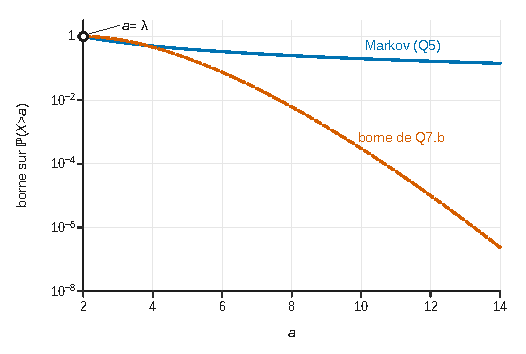
\includegraphics{figures/q7c-bornes-markov-chernoff.pdf}
\caption*{Figure 1 --- Bornes de Markov (Q5) et de Q7.b pour une loi de Poisson de
paramètre λ = 2, en échelle logarithmique : égales à 1 en a = λ, elles
se séparent ensuite très vite}
\end{figure}

\hypertarget{partie-iii-uxe9tude-dun-endomorphisme}{%
\section{Partie III : Étude d'un endomorphisme}\label{partie-iii-uxe9tude-dun-endomorphisme}}

\hypertarget{section-6}{%
\subsection{8.}\label{section-6}}

Soit \(\nu>0\), et soit \(P=\sum_{j=0}^n a_js^j\). Pour \(s\ge0\), on a :

\equationajustee{|P(s)|\le\sum_{j=0}^n|a_j|s^j .}

Par croissances comparées, \(s^je^{-s/(2\nu)}\to0\) quand \(s\to+\infty\), pour chaque \(j\). Par somme finie, \(|P(s)|e^{-s/(2\nu)}\to0\).

Par définition de la limite, appliquée avec \(\varepsilon=1\), il existe un réel \(M\ge0\) tel que \(|P(s)|e^{-s/(2\nu)}\le1\) pour tout \(s>M\). En multipliant par \(e^{-s/(2\nu)}>0\) :

\equationajustee{\boxed{\exists M\ge0,\ \forall s>M,\quad |P(s)|\,e^{-s/\nu}\le e^{-s/(2\nu)}.}}

\begin{figure}[H]
\centering
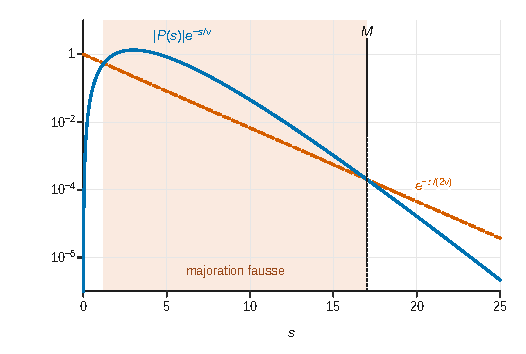
\includegraphics{figures/q8-domination-seuil-m.pdf}
\caption*{Figure 2 --- Exemple P(s) = s³ et ν = 1, en échelle logarithmique : la
majoration de Q8 est fausse pour 1,23 \textless{} s \textless{} 17,0 et
ne devient vraie qu'au-delà du seuil M ≈ 17}
\end{figure}

La fonction \(f:s\mapsto P(s)e^{-s/\nu}\) est continue sur \([0,+\infty[\). Le seul problème de convergence est donc en \(+\infty\).

\begin{itemize}
\tightlist
\item
  Sur le segment \([0,M]\), l'intégrale de \(f\) existe, par continuité.
\item
  Sur \([M,+\infty[\), la fonction positive \(|f|\) est majorée par la fonction positive \(s\mapsto e^{-s/(2\nu)}\), dont l'intégrale converge :
\end{itemize}

\equationajustee{\int_M^{+\infty}e^{-s/(2\nu)}\,\mathrm ds=\lim_{A\to+\infty}2\nu\left(e^{-M/(2\nu)}-e^{-A/(2\nu)}\right)=2\nu e^{-M/(2\nu)}.}

Par le critère de comparaison des intégrales de fonctions positives, \(\int_M^{+\infty}|f(s)|\,\mathrm ds\) converge. L'intégrale de \(f\) sur \([M,+\infty[\) converge donc absolument, donc converge. Par la relation de Chasles, \textbf{\(L_P(\nu)\) est bien défini}.

\hypertarget{section-7}{%
\subsection{9.}\label{section-7}}

Pour \(k\in\mathbb N\), posons \(J_k=\int_0^{+\infty}s^ke^{-s/\nu}\,\mathrm ds\). Cette intégrale converge par la question 8, appliquée au polynôme \(P=X^k\).

On montre par récurrence sur \(k\) la propriété \(\mathcal H_k\) : « \(J_k=k!\,\nu^{k+1}\) ».

\begin{itemize}
\tightlist
\item
  \textbf{Initialisation.} Pour \(A>0\), on a \(\int_0^Ae^{-s/\nu}\,\mathrm ds=\nu\left(1-e^{-A/\nu}\right)\), qui tend vers \(\nu\). Donc \(J_0=\nu=0!\,\nu^1\), et \(\mathcal H_0\) est vraie.
\item
  \textbf{Hérédité.} Soit \(k\ge1\) tel que \(\mathcal H_{k-1}\) soit vraie, et soit \(A>0\). On pose \(u(s)=s^k\) et \(v(s)=-\nu e^{-s/\nu}\).
\end{itemize}

Les fonctions \(u\) et \(v\) sont de classe \(\mathcal C^1\) sur \([0,A]\). Leurs dérivées sont \(u'(s)=ks^{k-1}\) et \(v'(s)=e^{-s/\nu}\).

Une intégration par parties sur le segment \([0,A]\) donne :

\equationajustee{\int_0^As^ke^{-s/\nu}\,\mathrm ds=\left[-\nu s^ke^{-s/\nu}\right]_0^A+k\nu\int_0^As^{k-1}e^{-s/\nu}\,\mathrm ds .}

Le crochet vaut \(-\nu A^ke^{-A/\nu}\), qui tend vers \(0\) quand \(A\to+\infty\), par croissances comparées. L'intégrale de droite tend vers \(J_{k-1}\). En faisant \(A\to+\infty\) :

\equationajustee{\begin{aligned}
J_k&=k\nu J_{k-1}\\
&=k\nu\cdot(k-1)!\,\nu^{k}\\
&=k!\,\nu^{k+1}.
\end{aligned}}

Donc \(\mathcal H_k\) est vraie. Par récurrence, \(\mathcal H_k\) est vraie pour tout \(k\in\mathbb N\). En divisant par \(\nu\) :

\equationajustee{\boxed{\forall k\in\mathbb N,\quad\frac1\nu\int_0^{+\infty}s^ke^{-s/\nu}\,\mathrm ds=k!\,\nu^k.}}

Si \(P=\sum_{k=0}^n a_kX^k\), la linéarité de l'intégrale s'applique, car \(L_P(\nu)\) est une somme finie d'intégrales convergentes :

\equationajustee{\boxed{L_P(\nu)=\sum_{k=0}^n k!\,a_k\,\nu^k.}}

\hypertarget{section-8}{%
\subsection{10.}\label{section-8}}

\textbf{\(L\) va de \(\mathbb R_d[X]\) dans \(\mathbb R_d[X]\).} L'écriture \(P=\sum_{k=0}^d a_kX^k\) dans la base \((1,X,\dots,X^d)\) est unique, donc \(L(P)\) est bien défini.

Le polynôme \(L(P)=\sum_{k=0}^d k!\,a_kX^k\) ne fait intervenir que des puissances \(X^k\) avec \(k\le d\). Il est donc de degré au plus \(d\), et appartient à \(\mathbb R_d[X]\).

\textbf{Linéarité.} Soient \(P=\sum_{k=0}^d a_kX^k\) et \(Q=\sum_{k=0}^d b_kX^k\) dans \(\mathbb R_d[X]\), et \(\mu\in\mathbb R\).

Le polynôme \(\mu P+Q\) s'écrit \(\sum_{k=0}^d(\mu a_k+b_k)X^k\) : ses coefficients sont les \(\mu a_k+b_k\). Par définition de \(L\) :

\equationajustee{\begin{aligned}
L(\mu P+Q)&=\sum_{k=0}^dk!\,(\mu a_k+b_k)X^k\\
&=\mu\sum_{k=0}^dk!\,a_kX^k+\sum_{k=0}^dk!\,b_kX^k\\
&=\mu L(P)+L(Q).
\end{aligned}}

\textbf{\(L\) est un endomorphisme de \(\mathbb R_d[X]\).}

\hypertarget{section-9}{%
\subsection{11.}\label{section-9}}

\equationajustee{\boxed{\dim\mathbb R_d[X]=d+1.}}

\hypertarget{section-10}{%
\subsection{12.}\label{section-10}}

Par définition, le noyau de \(L\) est l'ensemble des polynômes de \(\mathbb R_d[X]\) que \(L\) envoie sur le polynôme nul :

\equationajustee{\ker L=\{P\in\mathbb R_d[X]\ :\ L(P)=0\}.}

Soit \(P=\sum a_kX^k\). Un polynôme est nul si et seulement si tous ses coefficients sont nuls.

Donc \(L(P)=0\) équivaut à \(k!\,a_k=0\) pour tout \(k\).

Comme \(k!\neq0\), cela équivaut à \(a_k=0\) pour tout \(k\), soit \(P=0\). Donc :

\equationajustee{\boxed{\ker L=\{0\}.}}

\hypertarget{section-11}{%
\subsection{13.}\label{section-11}}

\(L\) est un endomorphisme injectif (question 12) de \(\mathbb R_d[X]\), espace de \textbf{dimension finie} \(d+1\) (question 11). Par le théorème du rang :

\equationajustee{\operatorname{rg}L=d+1-\dim\ker L=d+1 .}

Donc \(\operatorname{Im}L=\mathbb R_d[X]\).

\textbf{Oui, \(L\) est surjectif}, et même bijectif. On le voit aussi directement : \(\sum b_kX^k=L\left(\sum\frac{b_k}{k!}X^k\right)\).

\hypertarget{section-12}{%
\subsection{14.}\label{section-12}}

On a \(L(1)=1\), \(L(X)=X\), \(L(X^2)=2X^2\) et \(L(X^3)=6X^3\). Dans la base canonique \((1,X,X^2,X^3)\) :

\equationajustee{\boxed{\operatorname{Mat}(L)=\begin{pmatrix}1&0&0&0\\0&1&0&0\\0&0&2&0\\0&0&0&6\end{pmatrix}.}}

\hypertarget{section-13}{%
\subsection{15.}\label{section-13}}

Soit \(P=\sum_{k=0}^d a_kX^k\) et \(\mu\in\mathbb R\). En identifiant les coefficients, \(L(P)=\mu P\) équivaut à :

\equationajustee{\forall k\in\{0,\dots,d\},\quad(k!-\mu)\,a_k=0 .}

\begin{itemize}
\tightlist
\item
  Si \(\mu\) n'est égal à aucun des \(k!\), la seule solution est \(P=0\), et \(\mu\) n'est pas valeur propre.
\item
  Si \(\mu=k_0!\), les solutions sont les \(P\) dont les seuls coefficients non nuls sont ceux des \(X^k\) tels que \(k!=k_0!\).
\end{itemize}

Or \(0!=1!=1\), et \(k\mapsto k!\) est strictement croissante sur \(\mathbb N^*\). Les valeurs propres de \(L\) sont donc les \(k!\) pour \(0\le k\le d\) :

\equationajustee{\boxed{\operatorname{Sp}(L)=\{1,2,6,\dots,d!\}.}}

Les sous-espaces propres, engendrés par des polynômes, sont :

\equationajustee{\boxed{E_1(L)=\operatorname{Vect}(1,X)}}

de dimension \(2\), et, pour \(2\le k\le d\) :

\equationajustee{\boxed{E_{k!}(L)=\operatorname{Vect}(X^k).}}

Pour \(d=1\), on a \(\operatorname{Sp}(L)=\{1\}\) et \(L=\mathrm{id}\).

\hypertarget{section-14}{%
\subsection{16.}\label{section-14}}

Pour tout \(d\in\mathbb N^*\), la base canonique est formée de vecteurs propres de \(L\) : la matrice de \(L\) dans cette base est \(\mathrm{diag}(0!,1!,\dots,d!)\), qui est diagonale. De façon équivalente, la somme des dimensions des sous-espaces propres vaut \(2+(d-1)=d+1\).

\textbf{\(L\) est diagonalisable pour toute valeur de \(d\in\mathbb N^*\).}

\hypertarget{a.-1}{%
\subsection{17.a.}\label{a.-1}}

On vérifie les trois points de la caractérisation des sous-espaces vectoriels.

\begin{itemize}
\tightlist
\item
  \textbf{Inclusion.} Par définition, \(C(A)\) est formé de matrices de \(\mathcal M_3(\mathbb R)\), donc \(C(A)\subset\mathcal M_3(\mathbb R)\).
\item
  \textbf{Non vide.} La matrice nulle vérifie \(A\,0_3=0_3=0_3\,A\), donc \(0_3\in C(A)\).
\item
  \textbf{Stabilité par combinaison linéaire.} Soient \(M,N\in C(A)\) et \(\mu\in\mathbb R\). Par distributivité du produit matriciel, puis car \(AM=MA\) et \(AN=NA\) :
\end{itemize}

\equationajustee{\begin{aligned}
A(\mu M+N)&=\mu AM+AN\\
&=\mu MA+NA\\
&=(\mu M+N)A .
\end{aligned}}

Donc \(\mu M+N\in C(A)\).

\textbf{\(C(A)\) est un sous-espace vectoriel de \(\mathcal M_3(\mathbb R)\).}

\hypertarget{b.-1}{%
\subsection{17.b.}\label{b.-1}}

On calcule les deux produits :

\equationajustee{AM=\begin{pmatrix}0&0&0\\0&0&0\\g&h&k\end{pmatrix}}

et

\equationajustee{MA=\begin{pmatrix}0&0&c\\0&0&f\\0&0&k\end{pmatrix}.}

Deux matrices sont égales si et seulement si leurs neuf coefficients le sont. En identifiant, on obtient la condition nécessaire et suffisante :

\equationajustee{\boxed{M\in C(A)\iff(c,f,g,h)=(0,0,0,0).}}

Autrement dit, \(C(A)\) est l'ensemble des matrices de la forme \(\begin{pmatrix}a&b&0\\d&e&0\\0&0&k\end{pmatrix}\), avec \(a,b,d,e,k\) réels.

\hypertarget{c.-1}{%
\subsection{17.c.}\label{c.-1}}

Notons \(E_{i,j}\) les matrices élémentaires de \(\mathcal M_3(\mathbb R)\).

\equationajustee{\boxed{\text{Base de }C(A)\text{ : }(E_{1,1},E_{1,2},E_{2,1},E_{2,2},E_{3,3})}}

\equationajustee{\boxed{\dim C(A)=5.}}

\hypertarget{d.}{%
\subsection{17.d.}\label{d.}}

Pour \(\alpha,\beta\in\mathbb R\), \(\alpha I_3+\beta A=\mathrm{diag}(\alpha,\alpha,\alpha+\beta)\). Tout élément de \(\operatorname{Vect}(I_3,A)\) est donc diagonal.

Prenons \(M_0=E_{1,2}\), matrice dont l'unique coefficient non nul est un \(1\) en position \((1,2)\).

\begin{itemize}
\tightlist
\item
  On a \(M_0\in C(A)\), car ses coefficients \(c,f,g,h\) sont nuls (question 17.b).
\item
  On a \(M_0\notin\operatorname{Vect}(I_3,A)\), car son coefficient \((1,2)\) vaut \(1\neq0\) alors que \(M_0\) devrait être diagonale.
\end{itemize}

\equationajustee{\boxed{E_{1,2}=\begin{pmatrix}0&1&0\\0&0&0\\0&0&0\end{pmatrix}\in C(A)\setminus\operatorname{Vect}(I_3,A).}}

\hypertarget{partie-iv-loi-de-yulesimon}{%
\section{Partie IV : Loi de Yule--Simon}\label{partie-iv-loi-de-yulesimon}}

\hypertarget{section-15}{%
\subsection{18.}\label{section-15}}

Soit \(k\in\mathbb N\). La fonction \(f_k:s\mapsto(1-e^{-s})^ke^{-(\nu+1)s}\) est continue sur \([0,+\infty[\) : l'intégrale n'est généralisée qu'en \(+\infty\). Pour \(s\ge0\), on a \(0\le1-e^{-s}<1\), donc :

\equationajustee{0\le f_k(s)\le e^{-(\nu+1)s}.}

De plus, \(\int_0^{+\infty}e^{-(\nu+1)s}\,\mathrm ds\) converge, car \(\nu+1>0\), et vaut \(\frac1{\nu+1}\). Par le critère de comparaison des intégrales de fonctions positives, \textbf{l'intégrale définissant \(p_k\) converge}. On a de plus \(0\le p_k\le\frac\nu{\nu+1}\).

\hypertarget{section-16}{%
\subsection{19.}\label{section-16}}

Soit \(A>0\). La fonction \(\varphi:s\mapsto e^{-s}\) est de classe \(\mathcal C^1\) sur \([0,A]\), avec \(\varphi'(s)=-e^{-s}\).

Elle est strictement décroissante, de \([0,A]\) sur \([e^{-A},1]\). La fonction \(g:t\mapsto t^\nu(1-t)^k\) est continue sur \([e^{-A},1]\).

Pour \(s\in[0,A]\), on a \(1-e^{-s}=1-\varphi(s)\) et \(e^{-(\nu+1)s}=\varphi(s)^\nu\cdot\big(-\varphi'(s)\big)\). Le changement de variable \(t=\varphi(s)\) donne donc :

\equationajustee{\begin{aligned}
\int_0^A(1-e^{-s})^ke^{-(\nu+1)s}\,\mathrm ds&=-\int_0^Ag\big(\varphi(s)\big)\varphi'(s)\,\mathrm ds\\
&=-\int_1^{e^{-A}}t^{\nu}(1-t)^k\,\mathrm dt\\
&=\int_{e^{-A}}^1t^{\nu}(1-t)^k\,\mathrm dt .
\end{aligned}}

Quand \(A\to+\infty\), le membre de gauche tend vers \(p_k/\nu\) (question 18).

À droite, \(g\) est continue sur le segment \([0,1]\), car \(\nu>0\). La fonction \(x\mapsto\int_x^1g(t)\,\mathrm dt\) est donc continue en \(0\), et \(e^{-A}\to0\).

En multipliant par \(\nu\) :

\equationajustee{\boxed{\forall k\in\mathbb N,\quad p_k=\nu\int_0^1t^\nu(1-t)^k\,\mathrm dt.}}

\hypertarget{a.-2}{%
\subsection{20.a.}\label{a.-2}}

C'est une somme géométrique de raison \(1-t\). Cette raison vaut \(1\) seulement pour \(t=0\), cas qu'on traite à part.

\equationajustee{\boxed{\sum_{k=0}^N(1-t)^k=\begin{cases}\dfrac{1-(1-t)^{N+1}}{t}&\text{si }t\in\,]0,1],\\[2mm] N+1&\text{si }t=0.\end{cases}}}

Pour \(t=1\), la formule donne bien \(1\) : seul le terme \(k=0\) vaut \(1\), les autres sont nuls.

\hypertarget{b.-2}{%
\subsection{20.b.}\label{b.-2}}

Comme \(\nu-1>0\), la fonction \(t\mapsto t^{\nu-1}\) est croissante sur \(\mathbb R_+\). Pour \(t\in[0,1]\), on a donc :

\equationajustee{0\le t^{\nu-1}\le1^{\nu-1}=1 .}

On multiplie cette inégalité par le réel positif \((1-t)^{N+1}\) :

\equationajustee{0\le t^{\nu-1}(1-t)^{N+1}\le(1-t)^{N+1}.}

Les deux fonctions sont continues sur le segment \([0,1]\). Par croissance de l'intégrale :

\equationajustee{\boxed{\int_0^1t^{\nu-1}(1-t)^{N+1}\,\mathrm dt\le\int_0^1(1-t)^{N+1}\,\mathrm dt.}}

Le majorant vaut \(\left[-\frac{(1-t)^{N+2}}{N+2}\right]_0^1=\frac1{N+2}\).

\hypertarget{c.-2}{%
\subsection{20.c.}\label{c.-2}}

Il suffit de montrer que les \(p_k\) sont positifs et que \(\sum_{k=0}^{+\infty}p_k=1\). La positivité vient de la question 18.

Soit \(N\in\mathbb N\). Par la question 19 et la linéarité de l'intégrale (somme finie) :

\equationajustee{\begin{aligned}
\sum_{k=0}^Np_k&=\sum_{k=0}^N\nu\int_0^1t^\nu(1-t)^k\,\mathrm dt\\
&=\nu\int_0^1t^\nu\sum_{k=0}^N(1-t)^k\,\mathrm dt .
\end{aligned}}

Par 20.a, sur \(]0,1]\), on a :

\equationajustee{t^\nu\sum_{k=0}^N(1-t)^k=t^{\nu-1}\big(1-(1-t)^{N+1}\big).}

Les deux membres sont continus sur \([0,1]\) et valent \(0\) en \(t=0\), car \(\nu>1\). L'égalité vaut donc sur tout \([0,1]\), et :

\equationajustee{\begin{aligned}
\sum_{k=0}^Np_k&=\nu\int_0^1t^{\nu-1}\,\mathrm dt-\nu\int_0^1t^{\nu-1}(1-t)^{N+1}\,\mathrm dt\\
&=1-R_N,
\end{aligned}}

où l'on a posé :

\equationajustee{R_N=\nu\int_0^1t^{\nu-1}(1-t)^{N+1}\,\mathrm dt .}

Par 20.b, \(0\le R_N\le\frac\nu{N+2}\), qui tend vers \(0\). La série \(\sum p_k\) converge donc et sa somme vaut \(1\).

La suite \((p_k)_{k\in\mathbb N}\) est formée de réels positifs de somme \(1\) : c'est une loi de probabilité sur \(\mathbb N\). \textbf{Il existe donc une variable aléatoire discrète \(X\) telle que \(\mathbb P(X=k)=p_k\) pour tout \(k\in\mathbb N\).}

\hypertarget{partie-v-calculs-de-moments}{%
\section{Partie V : Calculs de moments}\label{partie-v-calculs-de-moments}}

Ici \(\nu>2\).

\hypertarget{a.-3}{%
\subsection{21.a.}\label{a.-3}}

Soient \(n,p\in\mathbb N\). Les fonctions \(u:t\mapsto\frac{t^{n+1}}{n+1}\) et \(v:t\mapsto(1-t)^{p+1}\) sont de classe \(\mathcal C^1\) sur \([0,1]\).

Leurs dérivées sont \(u'(t)=t^n\) et \(v'(t)=-(p+1)(1-t)^p\). On intègre par parties :

\equationajustee{I_{n,p+1}=\left[\frac{t^{n+1}}{n+1}(1-t)^{p+1}\right]_0^1+\frac{p+1}{n+1}\int_0^1t^{n+1}(1-t)^p\,\mathrm dt .}

Le crochet est nul aux deux bornes, car \(n+1\ge1\) et \(p+1\ge1\). Donc :

\equationajustee{\boxed{(n+1)\,I_{n,p+1}=(p+1)\,I_{n+1,p}.}}

\hypertarget{b.-3}{%
\subsection{21.b.}\label{b.-3}}

On montre par récurrence sur \(p\) la propriété \(\mathcal H_p\) : « pour tout \(n\in\mathbb N\), \(I_{n,p}=\frac{n!\,p!}{(n+p+1)!}\) ».

\begin{itemize}
\tightlist
\item
  \textbf{Initialisation.} Pour tout \(n\), \(I_{n,0}=\frac1{n+1}=\frac{n!\,0!}{(n+1)!}\), donc \(\mathcal H_0\) est vraie.
\item
  \textbf{Hérédité.} Supposons \(\mathcal H_p\) vraie et soit \(n\in\mathbb N\). On applique 21.a, puis \(\mathcal H_p\) à l'entier \(n+1\) :
\end{itemize}

\equationajustee{\begin{aligned}
I_{n,p+1}&=\frac{p+1}{n+1}\,I_{n+1,p}\\
&=\frac{p+1}{n+1}\cdot\frac{(n+1)!\,p!}{(n+p+2)!}\\
&=\frac{n!\,(p+1)!}{(n+(p+1)+1)!}.
\end{aligned}}

Donc \(\mathcal H_{p+1}\) est vraie. Par récurrence :

\equationajustee{\boxed{\forall n,p\in\mathbb N,\quad I_{n,p}=\frac{n!\,p!}{(n+p+1)!}.}}

\hypertarget{c.-3}{%
\subsection{21.c.}\label{c.-3}}

Par 21.b avec \(n=1\) et \(p=N\) :

\equationajustee{\begin{aligned}
(N+1)\int_0^1t(1-t)^N\,\mathrm dt&=(N+1)\,I_{1,N}\\
&=(N+1)\frac{N!}{(N+2)!}\\
&=\frac1{N+2}.
\end{aligned}}

Donc :

\equationajustee{\boxed{\lim_{N\to+\infty}(N+1)\int_0^1t(1-t)^N\,\mathrm dt=0.}}

\hypertarget{a.-4}{%
\subsection{22.a.}\label{a.-4}}

Soit \(N\in\mathbb N\). Pour \(t\neq0\), la raison \(1-t\) est différente de \(1\). La formule de 20.a vaut donc sur l'intervalle ouvert \(]0,2[\), qui contient \(]0,1]\) :

\equationajustee{\sum_{k=0}^N(1-t)^k=\frac{1-(1-t)^{N+1}}t .}

Les deux membres sont dérivables sur \(]0,2[\). On les dérive par rapport à \(t\), sans oublier le signe : la dérivée de \(t\mapsto(1-t)^k\) est \(t\mapsto-k(1-t)^{k-1}\).

À gauche, on obtient \(-\sum_{k=1}^Nk(1-t)^{k-1}\). À droite :

\equationajustee{\begin{aligned}
\frac{\mathrm d}{\mathrm dt}\left(\frac{1-(1-t)^{N+1}}t\right)&=\frac{(N+1)(1-t)^N\,t-\big(1-(1-t)^{N+1}\big)}{t^2}\\
&=\frac{(N+1)(1-t)^N}t-\frac1{t^2}+\frac{(1-t)^{N+1}}{t^2}.
\end{aligned}}

En changeant les signes, pour tout \(t\in\,]0,1]\) :

\equationajustee{\boxed{\sum_{k=1}^Nk(1-t)^{k-1}=\frac1{t^2}-\frac{(1-t)^{N+1}}{t^2}-\frac{(N+1)(1-t)^N}t.}}

\hypertarget{b.-4}{%
\subsection{22.b.}\label{b.-4}}

Le réel \(\nu\) n'est pas supposé entier : on ne peut pas utiliser la question 21, et l'on calcule directement. Comme \(\nu>2\), la fonction \(t\mapsto\nu t^{\nu-2}(1-t)\) est continue sur \([0,1]\), et :

\equationajustee{\begin{aligned}
\int_0^1\nu\,t^\nu(1-t)\frac1{t^2}\,\mathrm dt&=\nu\int_0^1\left(t^{\nu-2}-t^{\nu-1}\right)\mathrm dt\\
&=\nu\left(\frac1{\nu-1}-\frac1\nu\right)\\
&=\frac{\nu}{\nu-1}-1 .
\end{aligned}}

Sous forme de fraction irréductible :

\equationajustee{\boxed{\int_0^1\nu\,t^\nu(1-t)\frac1{t^2}\,\mathrm dt=\frac1{\nu-1}.}}

\hypertarget{c.-4}{%
\subsection{22.c.}\label{c.-4}}

Les termes \(kp_k\) sont positifs. \(X\) admet donc une espérance si et seulement si la suite des sommes partielles \(\Sigma_N=\sum_{k=1}^Nkp_k\) converge.

Par la question 19 et la linéarité (somme finie), en factorisant \((1-t)\) :

\equationajustee{\Sigma_N=\nu\int_0^1t^\nu(1-t)\sum_{k=1}^Nk(1-t)^{k-1}\,\mathrm dt .}

On remplace la somme par l'expression de 22.a, valable sur \(]0,1]\). On obtient :

\equationajustee{\Sigma_N=T-R_N^{(1)}-R_N^{(2)},}

où les trois termes valent :

\equationajustee{\begin{aligned}
T&=\nu\int_0^1t^{\nu-2}(1-t)\,\mathrm dt,\\
R_N^{(1)}&=\nu\int_0^1t^{\nu-2}(1-t)^{N+2}\,\mathrm dt,\\
R_N^{(2)}&=\nu(N+1)\int_0^1t^{\nu-1}(1-t)^{N+1}\,\mathrm dt.
\end{aligned}}

Les trois intégrandes sont continues sur \([0,1]\), car \(\nu-2>0\), ce qui justifie la séparation de l'intégrale. Les égalités ont lieu sur \(]0,1]\) et s'étendent en \(0\) par continuité.

\begin{itemize}
\tightlist
\item
  Par 22.b, \(T=\frac1{\nu-1}\).
\item
  Comme \(0\le t^{\nu-2}\le1\) sur \([0,1]\), on a \(0\le R_N^{(1)}\le\nu\int_0^1(1-t)^{N+2}\,\mathrm dt\). Ce majorant vaut \(\frac\nu{N+3}\) et tend vers \(0\).
\item
  Comme \(\nu-2>0\), on a \(t^{\nu-1}=t\cdot t^{\nu-2}\le t\) sur \([0,1]\). Avec \((1-t)^{N+1}\le(1-t)^N\), on obtient \(0\le R_N^{(2)}\le\nu\,(N+1)\int_0^1t(1-t)^N\,\mathrm dt\). Ce majorant tend vers \(0\) par 21.c.
\end{itemize}

Donc \(\Sigma_N\to\frac1{\nu-1}\), la série \(\sum kp_k\) converge, et \textbf{\(X\) admet une espérance} :

\equationajustee{\boxed{\mathbb E(X)=\frac1{\nu-1}.}}

\hypertarget{a.-5}{%
\subsection{23.a.}\label{a.-5}}

Pour \(t\in\,]0,1]\), on développe \((1-t)^2\) :

\equationajustee{\nu t^\nu(1-t)^2\frac2{t^3}=2\nu\left(t^{\nu-3}-2t^{\nu-2}+t^{\nu-1}\right).}

Comme \(\nu-3>-1\), l'intégrale \(\int_0^1t^{\nu-3}\,\mathrm dt\) converge et vaut \(\frac1{\nu-2}\). C'est une intégrale de Riemann en \(0\), généralisée si \(\nu<3\). Les deux autres termes sont continus sur \([0,1]\). Donc :

\equationajustee{\begin{aligned}
\mathbb E((X-1)X)&=2\nu\left(\frac1{\nu-2}-\frac2{\nu-1}+\frac1\nu\right)\\
&=2\nu\cdot\frac{\nu(\nu-1)-2\nu(\nu-2)+(\nu-1)(\nu-2)}{\nu(\nu-1)(\nu-2)}\\
&=2\nu\cdot\frac{2}{\nu(\nu-1)(\nu-2)}.
\end{aligned}}

Après simplification :

\equationajustee{\boxed{\mathbb E((X-1)X)=\frac4{(\nu-1)(\nu-2)}.}}

\hypertarget{b.-5}{%
\subsection{23.b.}\label{b.-5}}

On a \(X^2=(X-1)X+X\). Les variables \((X-1)X\) (énoncé) et \(X\) (question 22.c) admettent une espérance. Par linéarité, \(X^2\) admet une espérance. Donc \(X\) admet un moment d'ordre 2, et par conséquent une variance.

Par la formule de König--Huygens, \(\mathbb V(X)=\mathbb E(X^2)-\mathbb E(X)^2\), d'où :

\equationajustee{\begin{aligned}
\mathbb V(X)&=\mathbb E((X-1)X)+\mathbb E(X)-\mathbb E(X)^2\\
&=\frac4{(\nu-1)(\nu-2)}+\frac1{\nu-1}-\frac1{(\nu-1)^2}\\
&=\frac{4(\nu-1)+(\nu-1)(\nu-2)-(\nu-2)}{(\nu-1)^2(\nu-2)}.
\end{aligned}}

Le numérateur vaut \(4\nu-4+\nu^2-3\nu+2-\nu+2=\nu^2\), donc :

\equationajustee{\boxed{\mathbb V(X)=\frac{\nu^2}{(\nu-1)^2(\nu-2)}.}}

\hypertarget{c.-5}{%
\subsection{23.c.}\label{c.-5}}

Comme \(\mathbb E(X)>0\), on peut diviser :

\equationajustee{\frac{\mathbb V(X)}{\mathbb E(X)}=\frac{\nu^2}{(\nu-1)^2(\nu-2)}\cdot(\nu-1)=\frac{\nu^2}{(\nu-1)(\nu-2)}.}

Le dénominateur \((\nu-1)(\nu-2)\) est strictement positif, car \(\nu>2\). De plus :

\equationajustee{\nu^2-(\nu-1)(\nu-2)=3\nu-2>0 .}

Donc :

\equationajustee{\boxed{\frac{\mathbb V(X)}{\mathbb E(X)}=\frac{\nu^2}{(\nu-1)(\nu-2)}>1.}}

\hypertarget{section-17}{%
\subsection{24.}\label{section-17}}

Les deux modèles se distinguent par l'indice de dispersion \(\mathbb V(X)/\mathbb E(X)\) :

\begin{itemize}
\tightlist
\item
  dans la partie I (loi de Poisson), il vaut \(1\) (question 4). Pour la binomiale exacte \(\mathcal B(N,\lambda/N)\), il vaut \(1-\lambda/N\le1\) ;
\item
  dans la partie V (loi de Yule--Simon), il vaut \(\frac{\nu^2}{(\nu-1)(\nu-2)}>1\) (question 23.c), quel que soit \(\nu>2\).
\end{itemize}

À partir d'un échantillon \(x_1,\dots,x_n\) (nombres de bactéries survivantes dans \(n\) cultures indépendantes, menées dans les mêmes conditions), on calcule :

\begin{itemize}
\tightlist
\item
  la moyenne empirique \(\bar x=\frac1n\sum x_i\), qui estime \(\mathbb E(X)\) par la loi faible des grands nombres ;
\item
  la variance empirique \(s^2=\frac1{n-1}\sum(x_i-\bar x)^2\), estimation usuelle de \(\mathbb V(X)\) ;
\item
  puis l'indice empirique \(\widehat D=s^2/\bar x\).
\end{itemize}

\textbf{Règle :} si \(\widehat D\) est proche de \(1\), on privilégie le modèle de la partie I (mutations induites par l'exposition). Si \(\widehat D\) est nettement supérieur à \(1\) (sur-dispersion), on privilégie le modèle de la partie V (mutations spontanées transmises à la descendance). « Nettement » s'apprécie en fonction de la taille de l'échantillon.

\begin{figure}[H]
\centering
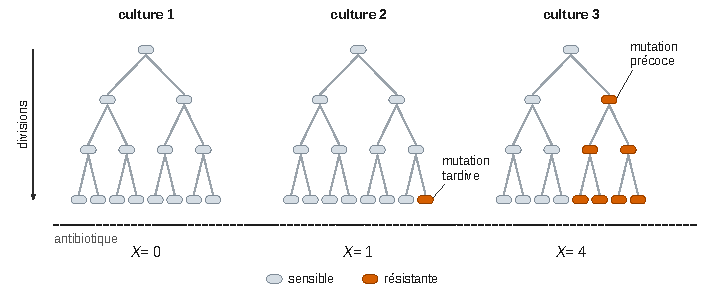
\includegraphics{figures/q24-mutations-cultures.pdf}
\caption*{Figure 3 --- Trois cultures parallèles : une mutation transmise à toute
la descendance donne 0, 1 ou 4 résistantes selon qu'elle est absente,
tardive ou précoce}
\end{figure}

\begin{figure}[H]
\centering
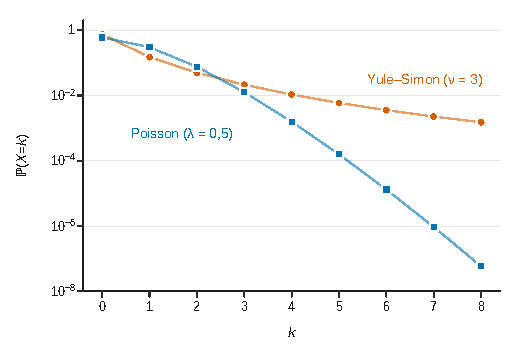
\includegraphics{figures/q24-poisson-yule-simon.pdf}
\caption*{Figure 4 --- Lois de Yule--Simon (ν = 3) et de Poisson (λ = 0,5), de
même espérance 0,5, en échelle logarithmique : la queue lourde de la
première porte l'indice de dispersion à 4,5}
\end{figure}

\end{document}
